\chapter{Quadtrees}
\label{app:quadtree}

The grid filter of \cref{ch:bayes} covers the lawn with cells of one
size, and the mask of \cref{fig:potato} marks each cell as on the lawn or
not. Most of these cells say nothing interesting: a cell deep inside the
lawn is on the lawn, and so are all its neighbours. The mask needs small
cells only along the edge, where the answer changes. A \emph{quadtree}
uses large cells where the answer is the same over a large region and
small ones along the edge. This appendix defines it
(\cref{sec:qt-def}), counts its cells (\cref{sec:qt-count}), shows how to
find the cell of a point (\cref{sec:qt-find}), and discusses a grid
filter whose cells are the cells of a quadtree (\cref{sec:qt-filter}).
The numbers quoted are printed by the script
\code{book/figures/make\_figures.py}, which also draws
\cref{fig:qtgrids,fig:qtchain,fig:qtclassify,fig:quadtree}.

\section{Splitting squares}
\label{sec:qt-def}

The lawn is a closed set $L$ in the plane, and its \emph{edge} is the
boundary of $L$: the outer edge, and the edge of each hole (the tree of
\cref{fig:potato}). A \emph{cell} is a closed square with sides parallel
to the axes. To \emph{split} a cell is to cut it through its centre,
parallel to its sides, into four cells of half the side, its
\emph{quadrants}.

\begin{definition}{Quadtree of a lawn}{quadtree}
Let $Q_0$ be a cell of side $s_0$ that contains $L$, and let
$h=s_0/2^m$ for an integer $m\ge1$. A cell is \emph{in} if all its points
are on the lawn, \emph{out} if none of them is, and \emph{mixed}
otherwise. Start from the single cell $Q_0$; as long as there is a mixed
cell of side larger than $h$, replace it by its four quadrants. The cells
left at the end are the \emph{leaves}. The \emph{quadtree} is the tree
whose nodes are all the cells met on the way, each split cell being the
parent of its four quadrants; $Q_0$ is its \emph{root}.
\end{definition}

\begin{figure}[t]
\centering
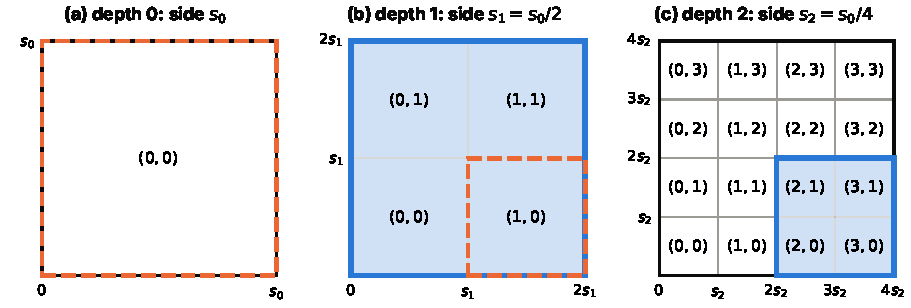
\includegraphics[width=0.8\linewidth]{figures/appE_quadtree_grids.pdf}
\caption{The grids of side $s_k$ on $Q_0$, each cell labelled by its
indices $(i,j)$: it is the square
$[\,i\,s_k,(i+1)\,s_k\,]\times[\,j\,s_k,(j+1)\,s_k\,]$. The dashed cell is
split; its quadrants (blue, inside the blue frame) are cells of the grid
of the next depth. (a)~$Q_0=(0,0)$ is split. (b)~Its quadrants are the
four cells of the grid of side $s_1$; the cell $(1,0)$ is split. (c)~Its
quadrants are the cells $(2,0)$, $(3,0)$, $(2,1)$, $(3,1)$ of the grid of
side $s_2$: the indices $(i,j)=(1,0)$ become $(2i,2j)$, $(2i+1,2j)$,
$(2i,2j+1)$ and $(2i+1,2j+1)$.}
\label{fig:qtgrids}

\vspace{1.5ex}
\centering
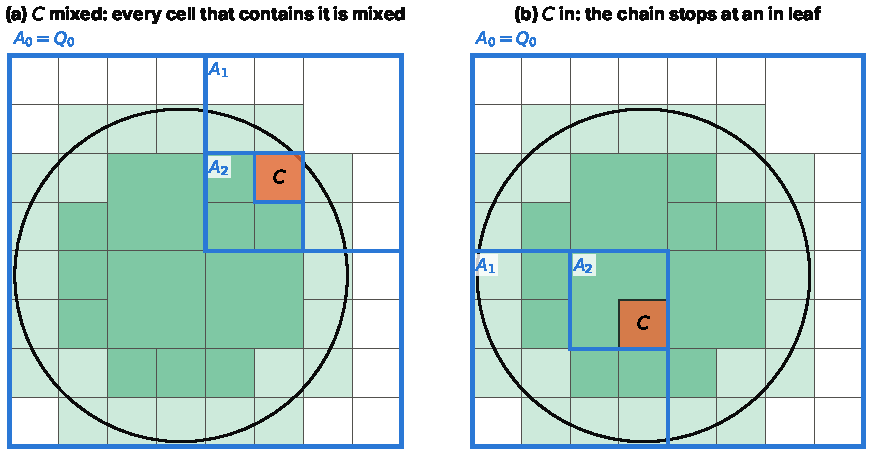
\includegraphics[width=0.75\linewidth]{figures/appE_quadtree_chain.pdf}
\caption{The cells of the quadtree that contain a cell $C$ of the uniform
grid of side $h$, on a round lawn with $Q_0$ of side $8h$: in leaves
(dark), mixed leaves (light), out leaves (white); the blue squares are
the chain $A_0\supset A_1\supset\dots$ (a) $C$ is mixed, so $A_1$ and
$A_2$, which contain it, are mixed and are split, down to $C$, which is a
leaf. (b) $C$ is in; $A_0$ and $A_1$ are mixed and split, and $A_2$, an
in leaf, is not split: $C$ lies inside it.}
\label{fig:qtchain}
\end{figure}

The cells of the construction all come from a few grids. Write $G_k$
for the uniform grid of side $s_k=s_0/2^k$ on $Q_0$: with the
coordinates measured from the lower-left corner of $Q_0$, its
$2^k\times2^k$ cells are the squares
\[
  [\,i\,s_k,(i+1)\,s_k\,]\times[\,j\,s_k,(j+1)\,s_k\,],
  \qquad 0\le i,j<2^k
\]
(\cref{fig:qtgrids}). The grid $G_m$, of side $s_m=h$, is the uniform
grid of \cref{ch:bayes}, and $G_0$ has the single cell $Q_0$. A cell is
\emph{at depth $k$} if it is obtained from $Q_0$ by $k$ splits.

\begin{proposition}{Basic properties of the quadtree}{qtbasic}
\begin{enumerate}[nosep,label=(\alph*)]
  \item A cell at depth $k$ has the side $s_k$. The construction stops,
        and no cell is deeper than $m$.
  \item The leaves cover $Q_0$, and two leaves overlap at most along
        their sides.
  \item Every cell at depth $k$ is a cell of the grid $G_k$.
  \item Every leaf is an in cell, an out cell, or a mixed cell of
        side $h$.
\end{enumerate}
\end{proposition}

\begin{proof}
(a) A split halves the side, so $k$ splits give the side $s_0/2^k=s_k$.
Only cells of side larger than $h=s_m$ are split, that is cells at depth
less than $m$, so no cell is deeper than $m$, and the construction ends.

(b) This is true at the start, when the only leaf is $Q_0$. A split
replaces a leaf by its four quadrants, which cover it and overlap only
along their sides, so it stays true after every split.

(c) At depth $0$, the only cell is $Q_0$, the cell of $G_0$. Suppose that
a cell at depth $k$ is the cell $(i,j)$ of $G_k$, the square above. Since
$s_k=2\,s_{k+1}$, its lower-left quadrant is
\[
  [\,2i\,s_{k+1},(2i+1)\,s_{k+1}\,]\times[\,2j\,s_{k+1},(2j+1)\,s_{k+1}\,],
\]
the cell $(2i,2j)$ of $G_{k+1}$, and the three others are the cells
$(2i+1,2j)$, $(2i,2j+1)$ and $(2i+1,2j+1)$ (\cref{fig:qtgrids}c). So the
cells at depth $k+1$ are cells of $G_{k+1}$ too, and the property holds
at every depth.

(d) A leaf is a cell that was not split. If it is mixed, it was not
split because its side is not larger than $h$, so by (a) its side is $h$.
\end{proof}

By (c), the quadtree never makes a cell that straddles two cells of these
grids: in \cref{fig:qtchain}, the cells of side $2h$ are cells of
$G_{m-1}$.

\emph{What the quadtree is for.} The mask of \cref{ch:bayes} is built on
$G_m$: each cell says ``lawn'' or ``not lawn''. The quadtree has far
fewer cells (\cref{sec:qt-count}). The next proposition shows that it
loses nothing: its leaves describe the lawn as well as the cells of
$G_m$.

\begin{proposition}{The quadtree is as precise as the uniform grid}{qtexact}
Let $C$ be a cell of $G_m$, the uniform grid of side $h$.
\begin{enumerate}[nosep,label=(\alph*)]
  \item If $C$ is mixed, $C$ is a leaf.
  \item If $C$ is in, it lies inside an in leaf; if $C$ is out, it lies
        inside an out leaf.
\end{enumerate}
Consequently, a mask on the leaves, built as in \cref{ch:bayes}, gives
the same answer at every point as the mask on $G_m$.
\end{proposition}

The idea: the quadtree keeps a large cell whole only when it is entirely
in or entirely out, and then all the cells of $G_m$ inside it have that
same status, so not splitting it loses nothing; where the lawn is mixed,
the quadtree splits down to the side $h$, like $G_m$.

\begin{proof}
\emph{Step 1: nested cells.} If a cell $B$ contains a cell $C$:
\begin{itemize}[nosep]
  \item if $C$ is mixed, so is $B$: $C$ has a lawn point and an off-lawn
        point, and both are points of $B$;
  \item if $B$ is in, so is $C$, and if $B$ is out, so is $C$: every point
        of $C$ is a point of $B$.
\end{itemize}

\emph{Step 2: the cells that can contain $C$.} For each depth $k$ from
$0$ to $m$, let $A_k$ be the cell of $G_k$ that contains $C$. Then
$A_0=Q_0$, $A_m=C$, and each $A_{k+1}$ is the quadrant of $A_k$ that
contains $C$:
\[
  Q_0=A_0\supset A_1\supset\dots\supset A_m=C .
\]
By \cref{prop:qtbasic}(c), the cells of the quadtree at depth $k$ are
cells of $G_k$, so the only cells of the quadtree that can contain $C$
are these $A_k$. The construction goes down this chain: it starts at
$A_0$, and whenever it splits $A_k$, the quadrant $A_{k+1}$ becomes a
cell of the tree.

\emph{Step 3: $C$ mixed} (\cref{fig:qtchain}a). Every $A_k$ contains $C$,
so by Step~1 every $A_k$ is mixed. Down the chain, each $A_k$ with $k<m$
is a mixed cell of side larger than $h$, so it is split and $A_{k+1}$
enters the tree. So $A_m=C$ enters the tree, and, having the side $h$, it
is not split: $C$ is a leaf. This proves (a).

\emph{Step 4: $C$ in} (\cref{fig:qtchain}b). Go down the chain while the
cells are split, and let $A_j$ be the first that is not: it is a leaf,
and it contains $C$. It is not mixed: by \cref{prop:qtbasic}(d) a mixed
leaf has the side $h$, so it would be $A_m=C$ itself, which is in. It is
not out either, since it contains the lawn points of $C$. So $A_j$ is an
in leaf that contains $C$. The same argument, with ``in'' and ``out''
exchanged, puts an out cell $C$ inside an out leaf. This proves (b).

\emph{Step 5: the two masks.} Take a point, and the cell $C$ of $G_m$
that contains it. If $C$ is mixed, it is itself a leaf by (a), marked in
the same way by both masks. If $C$ is in, both masks say ``lawn'': the
uniform grid through $C$, the quadtree through the in leaf that contains
$C$, by (b). If $C$ is out, both say ``not lawn''.
\end{proof}

\begin{figure}[t]
\centering
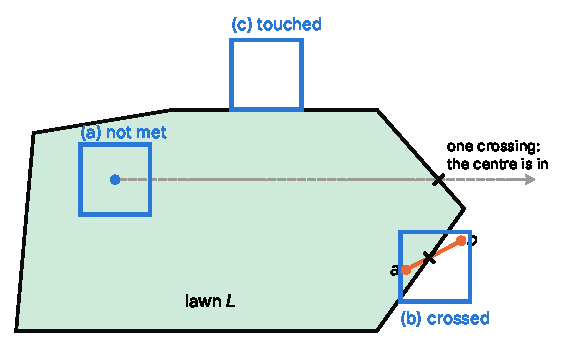
\includegraphics[width=0.72\linewidth]{figures/appE_quadtree_classify.pdf}
\caption{Classifying a cell against an edge that is a polygon. (a) The
edge does not meet the cell, so all its points have the status of the
centre; a half-line from the centre crosses the edge once, an odd number
of times, so the centre is on the lawn and the cell is in. (b) The edge
crosses the cell: the segment from the lawn point $a$ to the off-lawn
point $b$ meets the edge (cross) inside the cell; the cell is mixed.
(c) The edge only runs along a side of the cell, which is out; the rule
calls it mixed all the same.}
\label{fig:qtclassify}
\end{figure}

\begin{figure}[t]
\centering
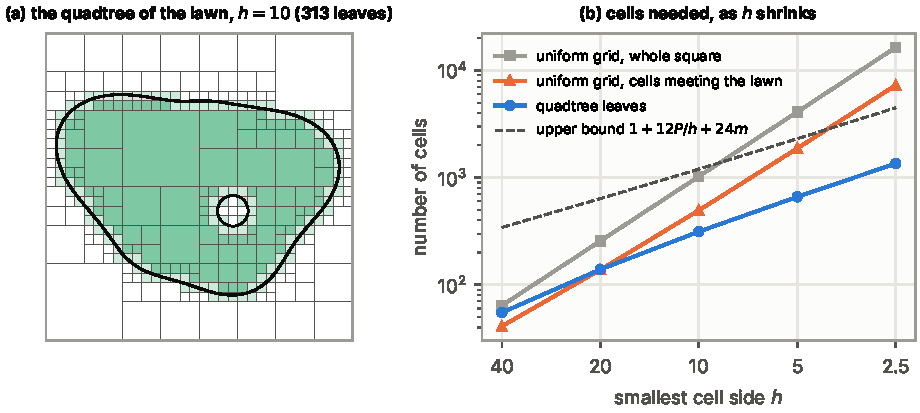
\includegraphics[width=\linewidth]{figures/appE_quadtree.pdf}
\caption{(a) The quadtree of the potato lawn of \cref{fig:potato}: a curved outer
edge, and a round tree (circle) inside, with
the root $Q_0=[-160,160]^2$ and the smallest side $h=10$: in leaves
(dark), mixed leaves (light), out leaves (white). (b) The number of cells
as the smallest side $h$ is halved: the uniform grid of side $h$ on the
whole square, its cells that meet the lawn, the leaves of the quadtree,
and the upper bound of \cref{prop:qtcount}.}
\label{fig:quadtree}
\end{figure}

\emph{Classifying a cell.} The construction must decide, for every cell
it meets, whether the cell is in, out or mixed. A cell has infinitely
many points, so they cannot all be tested; the edge gives the answer
instead. For a mower the edge is a polygon, recorded with the RTK GPS
(the box ``Boundary wire or geofence'' in \cref{ch:bayes}), and the
program uses this rule:
\begin{itemize}[nosep]
  \item if the edge meets the cell (one of the segments of the polygon
        meets the square), call the cell mixed;
  \item otherwise, test the centre of the cell, and call the cell in if
        the centre is on the lawn, out if it is not.
\end{itemize}
The test of the centre is the \emph{point-in-polygon test}: follow a
half-line from the point, and count how many times it crosses the
polygon; an odd number means that the point is inside, an even number
that it is outside, since each crossing goes in or out
(\cref{fig:qtclassify}a).

\emph{Why the rule is right.} It rests on one fact: \emph{a cell that the
edge does not meet is in or out}. Suppose that such a cell had a lawn
point $a$ and an off-lawn point $b$. The segment from $a$ to $b$ lies in
the cell, since a square contains the segment between any two of its
points. Going along it from $a$ to $b$, take the last point that is on
the lawn: it is on the lawn ($L$ is closed), and points just after it are
not, so it is a point of the edge, and it lies in the cell
(\cref{fig:qtclassify}b). That contradicts the assumption. So all the
points of the cell have the same status, which the centre gives. Two
consequences:
\begin{itemize}[nosep]
  \item every cell that the rule calls in or out is in or out, as called;
  \item every mixed cell meets the edge, so the rule calls it mixed.
\end{itemize}

\emph{Where the rule errs, and why it does not matter.} A cell that the
edge meets without crossing it, for example along one of its sides, is
in or out, but the rule calls it mixed (\cref{fig:qtclassify}c). If its
side is larger than $h$, it is split for nothing: its quadrants are
classified in turn, which costs a few leaves. If its side is $h$, it
stays a leaf called mixed, and the mask of \cref{ch:bayes}, by its centre
or by its fraction of lawn, still marks it correctly. So the quadtree
built with the rule may have a few more leaves, but its mask gives the
same answers. The rule is also the one of \cref{prop:qtcount}: split
every cell of side larger than $h$ that meets the edge. (For
\cref{fig:quadtree}, whose edges are given by formulas instead of a
polygon, the script uses tests suited to the formulas; its comments
explain them.)

\section{How many leaves}
\label{sec:qt-count}

A uniform grid of side $h$ has about $A/h^2$ cells on a lawn of area
$A$: halving $h$ multiplies their number by $4$. The leaves of a
quadtree are governed by the length of the edge instead.

\begin{proposition}{Number of leaves}{qtcount}
Suppose that the edge is made of $r$ closed curves of total length $P$,
and build the quadtree by splitting every cell of side larger than $h$
that meets the edge (this splits at least the mixed cells). Then the
number of leaves is at most
\[
  1+\frac{12P}{h}+12\,r\,m .
\]
\end{proposition}

\begin{proof}
\emph{Step 1: leaves and splits.} At the start there is one leaf. A split
removes one leaf and adds four, so it adds three. Hence
\[
  \text{number of leaves}=1+3\times\text{number of splits}.
\]

\emph{Step 2: a short arc meets at most four cells of a grid.} Fix a
side $s$ and the uniform grid of cells of side $s$. Let $\gamma$ be an
arc of length smaller than $s$. Any two of its points are at a distance
smaller than $s$, since the straight distance between two points is at
most the length of any curve that joins them. So the $x$-coordinates of
the points of $\gamma$ lie in an interval $[a,b]$ with $b-a<s$. The
interval $[js,(j+1)s]$ of the grid meets $[a,b]$ when $js\le b$ and
$(j+1)s\ge a$, that is when $a/s-1\le j\le b/s$; this interval of values
of $j$ has length $(b-a)/s+1<2$, so it contains at most two integers.
The same holds for the $y$-coordinates, and $\gamma$ meets at most
$2\times2=4$ cells.

\emph{Step 3: a curve meets few cells.} Cut a curve of length $\ell$
into $n=\lfloor\ell/s\rfloor+1$ arcs of equal length $\ell/n$, which is
smaller than $s$ because $n>\ell/s$. By Step~2 each arc meets at most $4$
cells, so the curve meets at most $4n\le4(\ell/s+1)$ cells. Adding over
the $r$ curves of the edge, whose lengths add up to $P$, at most
$4(P/s+r)$ cells of the grid of side $s$ meet the edge.

\emph{Step 4: adding over the depths.} The split cells have the sides
$s_k=s_0/2^k$ with $0\le k\le m-1$, and at each depth they are cells of
the grid of side $s_k$ that meet the edge, so by Step~3 there are at most
$4(P/s_k+r)$ of them. The sum of the $1/s_k$ is a geometric sum:
\[
  \sum_{k=0}^{m-1}\frac1{s_k}=\frac1{s_0}\sum_{k=0}^{m-1}2^k
  =\frac{2^m-1}{s_0}=\frac1h-\frac1{s_0}<\frac1h ,
\]
using $s_0=2^mh$. Hence
\[
  \text{number of splits}\le\sum_{k=0}^{m-1}4\Bigl(\frac P{s_k}+r\Bigr)
  <\frac{4P}h+4rm ,
\]
and Step~1 gives the bound.
\end{proof}

\begin{inwords}
The leaves are about the edge, not about the area. Halving $h$ about
doubles the bound on the number of leaves, where it quadruples the number
of cells of a uniform grid. The term $12rm$ grows only like the
logarithm of $s_0/h$.
\end{inwords}

\emph{The potato lawn.} Its edge is the outer curve, of length $798.7$,
and the edge of the tree, of length $2\pi\times16=100.5$: $r=2$ and
$P=899.2$. The area of the lawn is $A=44\,084$, and $s_0=320$.
\begin{center}
\small
\begin{tabular}{@{}rrrrr@{}}
\toprule
 & quadtree & \multicolumn{2}{c}{uniform grid} & bound of\\
\cmidrule(lr){3-4}
$h$ & leaves & whole square & cells meeting the lawn &
\cref{prop:qtcount}\\
\midrule
$40$  & $55$    & $64$     & $41$    & $343$\\
$20$  & $139$   & $256$    & $138$   & $637$\\
$10$  & $313$   & $1\,024$ & $494$   & $1\,200$\\
$5$   & $661$   & $4\,096$ & $1\,871$ & $2\,303$\\
$2.5$ & $1\,351$ & $16\,384$ & $7\,277$ & $4\,485$\\
\bottomrule
\end{tabular}
\end{center}
For large cells the quadtree gains nothing: almost every cell is near the
edge. Each halving of $h$ then about doubles the number of leaves and
quadruples the number of lawn cells of the uniform grid (\cref{fig:quadtree}b), so the ratio doubles: $1.6$ at $h=10$, $2.8$ at $h=5$, $5.4$ at
$h=2.5$.

The bound is about three times too large. Step~2 allows four cells per
arc of length $s$, the worst case; a typical arc of length $s$ meets
fewer. The script finds between $1.25\,P/h$ and $1.29\,P/h$ mixed leaves
at the values of $h$ of the table. This agrees with a classical result of integral geometry,
quoted here without proof (it is Buffon's needle problem): averaged over
the position and orientation of a grid of side $s$, a curve of length
$\ell$ crosses $2\ell/(\pi s)$ of its vertical lines and as many
horizontal ones, and each crossing takes it into a new cell, which gives
about $4P/(\pi h)\approx1.27\,P/h$ cells along the edge. Putting this
count in Step~4 instead of $4P/s_k$ gives about
$1+3\times1.27\,P/h\approx3.8\,P/h$ leaves: about $1\,370$ for $h=2.5$,
against $1\,351$ in the table.

A leaf costs more memory than a cell of a uniform grid, which is an
entry of an array: it needs its position and size, or the links of the
tree. The quadtree pays off when the cells are small compared with the
lawn, that is when $h$ is much smaller than $A/P$ (here $49$), which is
when $A/h^2$ is much larger than $P/h$.

\section{Finding the leaf of a point}
\label{sec:qt-find}

To find the leaf that contains a point $\p$, start at the root; at a
cell that has been split, compare the coordinates of $\p$ with those of
the centre of the cell, which tells in which quadrant $\p$ lies (two
comparisons), and move to that quadrant; stop at a leaf. Each step goes
one level down, so at most $m=\log_2(s_0/h)$ steps are needed: $7$ for
$h=2.5$. A uniform grid finds the cell of $\p$ in one step, by dividing
its coordinates by $h$, but it stores $A/h^2$ cells. This is the trade:
memory proportional to $P/h$ for a search in $\log_2(s_0/h)$ steps.

The particle filter of \cref{ch:particle} needs exactly this search: a
particle in an out leaf is off the lawn and gets zero likelihood, a
particle in an in leaf is on the lawn, and only for a particle in a mixed
leaf is a finer test needed, against the pieces of the edge that cross
that leaf. In three dimensions, the same construction with eight
children per cell is the \emph{octree}, on which the OctoMap library
builds its 3-D occupancy maps (Hornung et al., in the references).

\section{A grid filter on a quadtree}
\label{sec:qt-filter}

The grid filter can use the leaves as its cells. The belief is a
probability $b_\ell$ for each leaf $\ell$, spread evenly inside the leaf,
as on a uniform grid; the out leaves have $b_\ell=0$ and need not be
stored. Write $\vect c_\ell$ for the centre of the leaf $\ell$.

\emph{Update.} As in \cref{ch:bayes}, $b_\ell\leftarrow\eta\,
p(\z\mid\vect c_\ell)\,b_\ell$, with $\eta$ chosen so that the $b_\ell$
add up to $1$. Taking the likelihood at the centre replaces its average
over the leaf by one value, which is accurate when the likelihood
changes little across the leaf.

\emph{Prediction.} By the law of total probability over the leaf that
contains $\p_t$ (the version of \eqref{eq:predict} for cells),
$\bar b_{\ell'}=\sum_\ell T_{\ell\ell'}\,b_\ell$ with
$T_{\ell\ell'}=\Pr(\p_{t+1}\in\ell'\mid\p_t\in\ell)$. Take the model of
\cref{prop:conv} with the round noise $\Normal(\vect0,\sigma^2I)$ used by
the code, and put the robot at the centre of its leaf. Then $\p_{t+1}$
is Gaussian with the mean $\vect\mu=\vect c_\ell+\vect d_t$ and the
covariance $\sigma^2I$. Its two coordinates are independent, because the
covariance is diagonal, and for a Gaussian $X$ with mean $\mu$ and
standard deviation $\sigma$,
$\Pr(a\le X\le b)=\Phi\bigl((b-\mu)/\sigma\bigr)-\Phi\bigl((a-\mu)/\sigma\bigr)$,
where $\Phi$ is the distribution function of the standard Gaussian. So,
for the leaf $\ell'=[x_0,x_1]\times[y_0,y_1]$,
\[
  T_{\ell\ell'}=
  \Bigl[\Phi\Bigl(\frac{x_1-\mu_x}{\sigma}\Bigr)
       -\Phi\Bigl(\frac{x_0-\mu_x}{\sigma}\Bigr)\Bigr]
  \Bigl[\Phi\Bigl(\frac{y_1-\mu_y}{\sigma}\Bigr)
       -\Phi\Bigl(\frac{y_0-\mu_y}{\sigma}\Bigr)\Bigr].
\]
Only the leaves $\ell'$ near $\vect\mu$ receive anything: if $\ell'$
lies entirely more than $4\sigma$ to the right of $\mu_x$, the first
factor is at most $1-\Phi(4)=\Phi(-4)\approx3\times10^{-5}$, and the same
holds on the other three sides. The probability sent to out leaves is
dropped and the rest is renormalised, which is the mask of
\cref{ch:bayes}. On a uniform grid the same formula is the shift and the
blur of \cref{prop:conv}, done cell by cell.

\emph{The weakness.} Both steps put the robot at the centre of its leaf,
so they are only as fine as the leaves. The quadtree of the lawn has its
small leaves along the edge, which is where the \emph{map} needs detail,
but large leaves inside the lawn, where the robot spends most of its
time. A belief concentrated on a few units cannot be represented inside
a leaf of side $40$: there it is spread evenly over the whole leaf. The resolution of the
belief should follow the \emph{belief}. One way is to let the
probabilities drive the splitting: after each update, split a leaf whose
probability is above a threshold, down to the side $h$, and merge four
sibling leaves whose total probability is below another threshold. The
mask still decides which leaves are out, and a leaf is split when it is
mixed or when it carries much probability. Thrun, Burgard and Fox call a
decomposition fixed in advance \emph{static} and one that follows the
belief \emph{dynamic} (Section~4.1.4 of \emph{Probabilistic Robotics},
where the dynamic decomposition is a \emph{density tree}). They also
describe a simpler variant, \emph{selective updating}: keep the uniform
grid, but update only the cells whose probability is above a threshold.
The
particle filter of \cref{ch:particle} reaches the same goal by other
means: its particles gather where the belief is, and the quadtree is then
used only for the map, as in \cref{sec:qt-find}.
